\documentclass[12pt,a4paper,english]{beamer}
\usepackage{ucs}
\usepackage[latin1]{inputenc}%utf-8 utf8x
%\usepackage{lmodern}
\usepackage{fontenc}%[T1]
\usepackage{babel}%[T1]
\usepackage{amssymb,amsmath,wick}
\usepackage{epsfig}
\usepackage{wrapfig}
\usepackage{color,subfigure}  
\usepackage{beamerthemesplit}
\usepackage{graphicx}
\usepackage{listings}
%\usepackage[pdftex,colorlinks=true,bookmarks=true,linkcolor=blue]{hyperref}
\let\Tiny=\tiny

\newcommand{\be}{ \begin{equation}}
\newcommand{\ee}{ \end{equation}}
\newcommand{\mc}{ \mathcal }
\newcommand{\mbf}{ \mathbf }
\newcommand{\bra}[1]{\langle #1|}
\newcommand{\ket}[1]{|#1\rangle}
\newcommand{\braket}[2]{\langle #1|#2\rangle}
\newcommand{\braopket}[3]{\langle #1|#2|#3\rangle}
\newcommand{\beq}{\begin{equation*}}
\newcommand{\eeq}{\end{equation*}}
\newcommand{\ds}{\displaystyle{\not}}
\newcommand{\matr}[1]{{\bf \cal{#1}}}
\newcommand{\OP}[1]{{\bf\widehat{#1}}}


\title{PBC in LSDALTON}
\begin{document}
\date{}
%\author{Johannes Rekkedal}
\frame{\titlepage}
%\section{Outline}
\begin{frame}
        \frametitle{Outline}
  \tableofcontents
\end{frame}

%\section{Shcr\"odinger equation}
%\begin{frame}
%  The Hamiltionian
%  \begin{equation}
%	H= \sum_i \frac{\nabla^2_i}{2} + \sum_{A}\frac{Z_A}{r-R_A}+\sum_{i>j}\frac{1}{r_{ij}}
%	\label{eq:ham}
%  \end{equation}
%
%\end{frame}

\section{Periodicity and the Hamiltonian}

\begin{frame}
 Crystalline solids can be described as ordered repetitions of atoms or groups
 of atoms. In an ideal crystal all repeating units are 
 identical and they can be related to each other by the lattice vector
 \begin{equation*}
   \mbf R_n= u\mbf t_1 + v\mbf t_2 + w\mbf t_3
 \end{equation*}
 $u,v~\mbox{and}~w\in \mathbb{Z}$
%\end{frame}
%
%\begin{frame}
\\ The vectors $\mbf t_i$ are three vectors defining the
 basis of the space.
 The parallelepiped formed by these three vectors is called the unit cell and
 their direction define the crystallographic axes $X,~Y~\mbox{and}~Z$.
\end{frame}

%\section{Bravais lattices}

\begin{frame}
  In three dimensions there are 14 different Bravais lattices classified in 7
  crystal systems.

  \begin{figure}[htp]
\centering
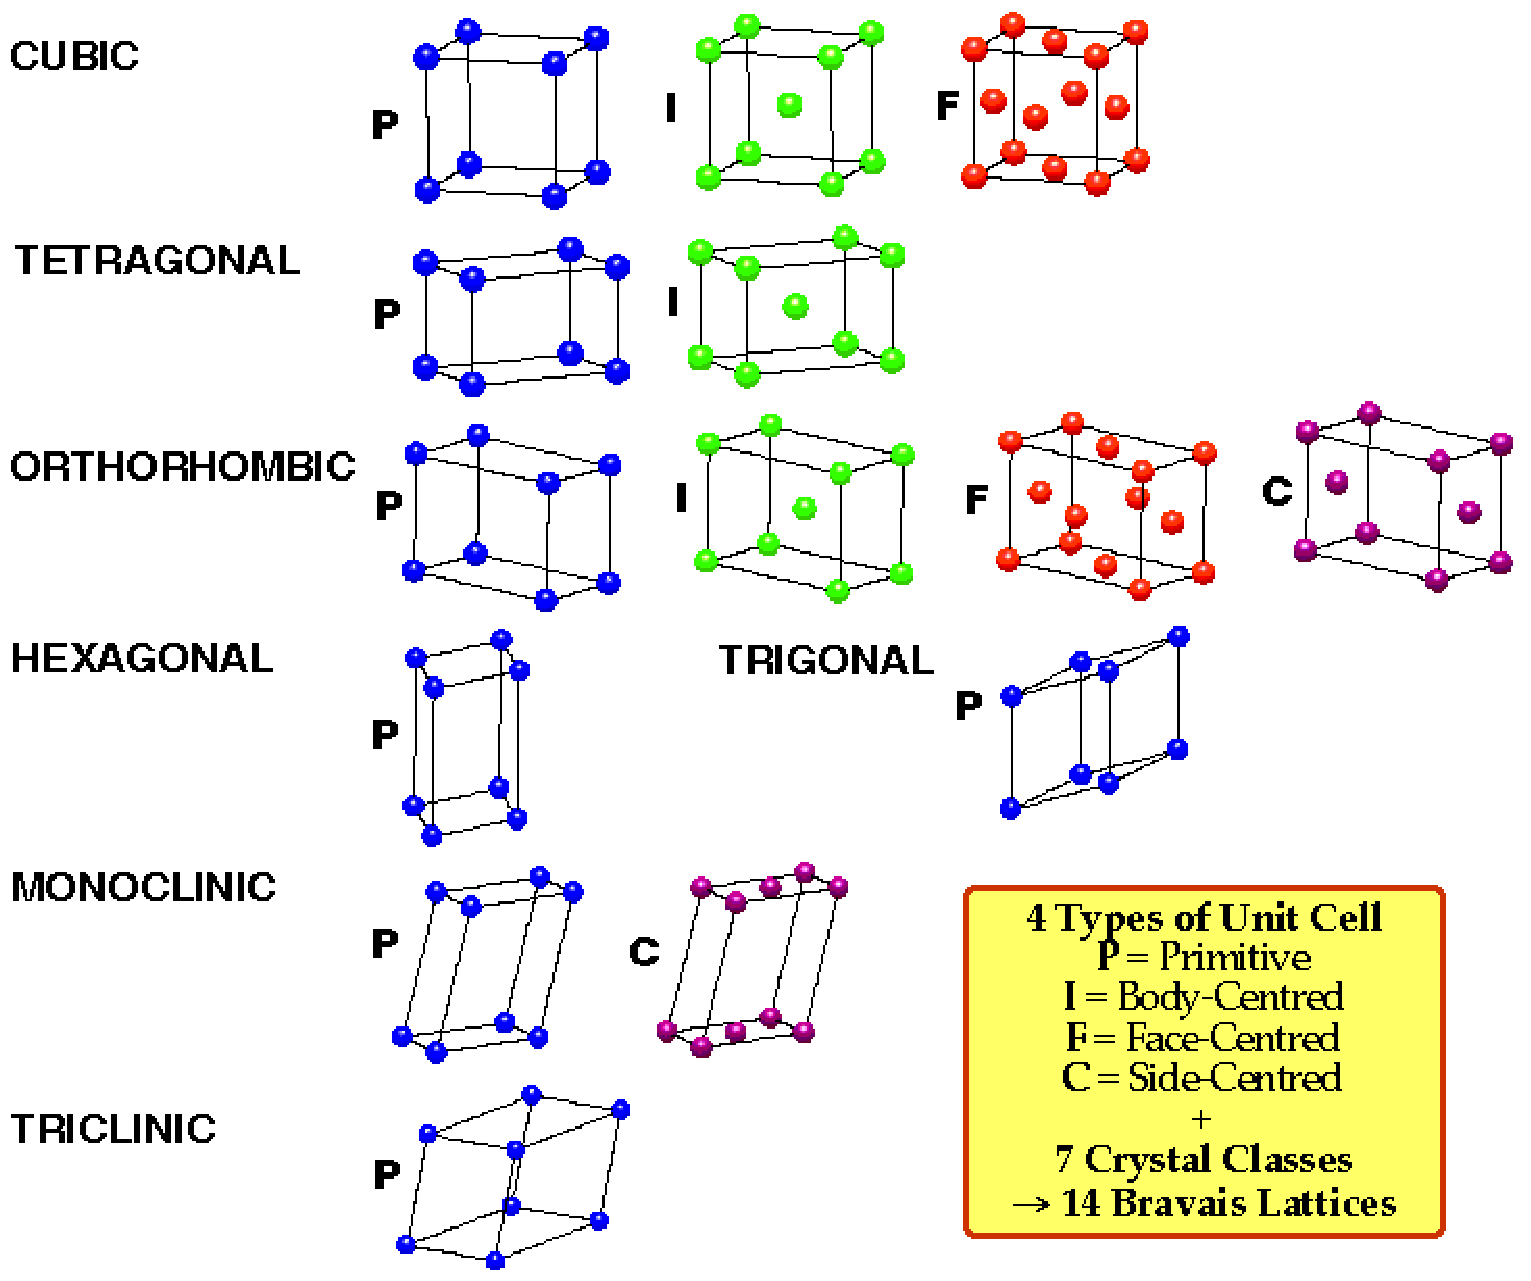
\includegraphics[scale=0.3]{Bravais}
\caption{The 14 different Bravais lattices and the 7 crystal systems.}
\label{fig:bravais}
\end{figure}
\end{frame}

\begin{frame}
  \emph{The set of all vectors $\mbf{K}$ that yield plane waves with the periodicity of a given lattice is known as its reciprocal lattice.}
  $$e^{iK(r+R_n)}=e^{iKr}.$$
  The reciprocal lattice can be generated by three primitive vectors $\mbf g_i$
  defined by the relation 
  $$\mbf t_i\cdot \mbf g_j=2\pi\delta_{ij}.$$

  Any vector in the reciprocal lattice can be written as a linear combination of  the $\mbf g_i.$
  $$\mbf k= \sum_{i=1}^3 k_i\mbf g_i.$$

\end{frame}

%\begin{frame}
%  With a periodic Hamiltonian,
%  $$H=\frac{\mbf p^2}{2m}+v(\mbf r)$$
%  $$v(\mbf r+\mbf R_n)=v(\mbf r).$$
%  the potential may be expanded in terms of the reciprocal
%  vectors $\mbf G_m=m_1\mbf g_1+m_2\mbf g_2+m_3\mbf g_3$
%  $$v(\mbf r)=\sum_mv(\mbf G_m)e^{i\mbf G_m\mbf r.}$$
%\end{frame}

\begin{frame}
  The eigenfunctions to a periodic Hamiltonian, where $H(r+R)=H(r)$, are the so called Bloch functions
  $$\psi_{\mu\mbf k}(\mbf r)=e^{i\mbf k\mbf r}u_{\mu\mbf k}(\mbf r),$$ where $u_{\mu\mbf k}(\mbf r)$ is periodic in $\mbf r.$ It is easy to see that the wavefunction has the property
  $$\psi_{\mu\mbf k}(\mbf r+\mbf R_n)=e^{i\mbf k\mbf R_n}\psi_{\mu\mbf k}(\mbf r).$$

  The Schr\"odinger equation for a Bloch function gives us the so called 
  band-energies, ie. energy levels, $\mu$, that are dependent on the 
  parameter $k.$
  $$H\psi_{\mu\mbf k}=\varepsilon_{\mu,k}\psi_{\mu\mbf k}.$$
%  \begin{equation*}
%		  \left[\frac{1}{2}\left(-i\nabla+\mbf k\right)^2+V(\mbf r)\right]\psi_{\mu k}(\mbf r)=\varepsilon_{\mu}(\mbf k)\psi_{\mu k}(\mbf r)
%  \end{equation*} 
\end{frame}

%\section{Hartree Fock with Bloch functions}
\begin{frame}

	   The self consistent field equations are solved 
	   for each $k$ value in the first Brillouin zone:
		\begin{equation*}
				F(k)C(k)=\varepsilon(k)S(k)C(k),
		\end{equation*}

		where
		\begin{equation}
		  F_{\mu\nu}(k)=h_{\mu\nu}(k)+J_{\mu\nu}(k) + K_{\mu\nu}(k)
		  \label{eq:kspacefock}
		\end{equation}


\end{frame}

%\begin{frame}[fragile]
%  \begin{itemize}
%	\item The connection with LSDalton is in the computation of the integrals 
%  which are all done in realspace.
%
%\item In the pbc code we loop over all lattice cells that are necessary in the 
\section{Plane waves and Gaussians}
\begin{frame}
  Plane waves
  \begin{itemize}
	\item A complete and orthonormal set.
	\item Does not depend on the positions of the atoms in the unit cell.
	\item Fast Fourier transforms are easy to program.
	\item Forces on atoms are easy to compute
	\item Plane waves do not suffer from basis set superposition error.
	\item In practice we must use a finite set of plane waves, core states are thus described badly, must augment the basis set or use pseudo potentials.
  \end{itemize}
\end{frame}
\begin{frame}
  Gaussians
  \begin{itemize}
	\item Allows to describe accurately electronic distributions both in valence and the core region with a limited number of basis functions.
	\item Allows a treatment of both finite and infinite systems in one two or three dimensions.
	\item Integrals can be done analytically.
	\item Linear scaling
  \end{itemize}
\end{frame}

\begin{frame}

  While using Gaussians as basis functions, the $k$ dependency of the Fock matrix is given by the fourier transformation
  \begin{equation}
	F_{\mu\nu}(k)=\sum_{\mbf j}e^{ikj}F_{\mu\nu}^{0j},
	   \label{hfbleq:totmatx2}
	 \end{equation}
	 where $j$ is a lattice vector and
	 \begin{equation}
	   F_{\mu\nu}^{0j}=h_{\mu\nu}^{0j}+J_{\mu\nu}^{0j}+K_{\mu\nu}^{0j}.
	 \end{equation}

	 Each part of the fock matrix has first to be computed in real space.

\end{frame}
\begin{frame}[fragile]

  A pseudo-code for the kinetic energy:

\begin{lstlisting}
DO index=1,num_latvectors
 call TYPEDEF_setmolecules(setting,refcell,1,&
 &                        latt_cell(index),3)

 call II_get_kinetic(lupri,luerr,setting,kin)
ENDDO
\end{lstlisting}
  
  %The one-particle operator part is given by
  %$$h_{\mu\nu}^{0j}=\braopket{\chi_{\mu}^0}{\hat h}{\chi_{\nu}^j}$$
  %where the superscript $0$ indicates that the basis function has center in the   reference cell and $j$ that the basis function has center in the cell $j$.
  



\end{frame}

\section{Integrals} \begin{frame} The bottleneck in the calculations are the
        two-body integrals. \\
        \vspace{\baselineskip}
        The Coulomb integral is speed up in the LSDALTON program by using the 
        j-engine algorithm. \\
        \vspace{\baselineskip}
        The coulomb integral $J_{ab}$, written as a sum over primitive coulomb integrals
        $J_{ab}=\sum_{ij}J_{[a_ib_j]}$
                
        \begin{equation}
        \begin{split}
                %&J_{ab}=\sum_{cd}(ab|cd)D_{cd}=\sum_{cd}\sum_{mnij}C_{mn}C_{ij}[a_mb_n|c_id_j]D_{cd}\\
                %&=\sum_{cd}\sum_{mnij}\sum_{qr}C_{mn}C_{ij}E^{mn}_{q}E^{ij}_q[q|r]D_{cd}\\
                %&=\sum_{mn}C_{mn}\sum_qE^{mn}_q\sum_r F^{ij}_{r}[q|r]
                &J_{a_ib_j}=\sum_{mn}\rho^{c_md_n}[a_ib_j|c_md_n]\\
                %&=\sum_{p}E^p_{ab}\sum_{mn}\rho^{c_md_n}[p|c_md_n]\\
                %&=\sum_{mn}\rho^{c_md_n}[a_ib_j|c_md_n]\\
                &=\sum_{mn}\sum_q\rho^{c_md_n}E^q_{c_md_n}[a_ib_j|q]\\
        \end{split}
                %&(ab|cd)=\sum_{mnij}C_{mn}C_{ij}[a_mb_n|c_id_j]D_{cd}\\
                %&=\sum_{mnij}\sum_{qr}C_{mn}C_{ij}E^{mn}_{q}E^{ij}_q[q|r]\\
                %&=\sum_{mn}C_{mn}\sum_qE^{mn}_q\sum_r F^{ij}_{r}[q|r]
        \end{equation}
\end{frame}
\begin{frame}
        The sum over $m$ and $n$ are independent of the integral and can be presummed with the conditions that $c_m$ and $d_n$ are belonging to the center $q$.
        \begin{equation}
                \begin{split}
                        &[p|CD]=\sum_{mn}\rho^{c_md_n}[p|c_md_n]\\
                        &=\sum_{mn}\sum_q\rho^{c_md_n}E^q_{c_md_n}[p|q]\\
                        &=\sum_q\rho^q[p|q]
                \end{split}
                \label{}
        \end{equation}
        where
        \begin{equation}
                \rho^q=\sum_{mn}\rho^{c_md_n}E^q_{c_mc_n}
                \label{}
        \end{equation}
\end{frame}

%\begin{frame}
%        Exact exchange is computed using the Linear exchange K, LinK, scheme. 
%\end{frame}

%  fourier transform, and call the integrals in LSDalton.
%  \end{itemize}
%
\begin{frame}
        \begin{table}
                \centering
                \begin{tabular}{|c|c|c|c|}
                         Iteration & K&J&Total time (sec) \\
\hline
                         1 & 1.21 & 0.50 &1.71\\ 
                         2 & 1.99 & 0.51 &2.48\\ 
                         3 & 1.40 & 0.51 &1.91\\ 
                         4 & 1.40 & 0.51 &1.91\\ 
                         5 & 1.43 & 0.52 &1.95\\ 
                         6 & 1.21 & 0.51 &1.72\\ 
                         7 & 1.33 & 0.52 &1.75\\ 
                         8 & 1.20 & 0.51 &1.71\\ 
                         9 & 1.21 & 0.51 &1.72\\ 
                        10 & 1.21 & 0.51 &1.72\\ 
                        11 & 1.20 & 0.51 &1.71\\ 
                        12 & 1.21 & 0.51 &1.72\\ 
                \end{tabular}
                \caption{Total time for computation of J and K for water in a 6-31G** basis}
                \label{tab:1}
        \end{table}          
\end{frame}
  
  
  
  
  
  
  
  
  
  
  
   

%\section{PBC in LSDALTON}
%\begin{frame}
%  In order to use the pbc code, there are two important things which have to be  included in the MOLECULE.INP file.
%  The keyword \emph{PBC} either in capital or small letters, has to be specified together on the same foothing as the the atomtypes, and charge, while the lattice deciding the periocity of the system 
%  has to be setup below the geometry of the molecule. 
%
%\end{frame}
%
%  \begin{frame}[fragile]
%	\frametitle{An example of a MOLECULE.INP file}
%  \begin{lstlisting}
%  BASIS
%4-31G Aux=Ahlrichs-Coulomb-Fit
%LDA molecular hessian without symmetry
%Ethane LDA molecular hessian without symmetry
%Atomtypes=1 Charge=0 Nosymmetry PBC
%        1.    2
%H  4.6000000000    0.0000000000     0.0000000
%H -4.6000000000    0.0000000000     0.0000000
%a1 = 10.0 0.0 0.0 active 
%a2 = 0.0 10.0 0.0 active
%a3 = 0.0 0.0 10.0 inactive
%  \end{lstlisting}
%\end{frame}
%  
%  \begin{frame}
%	The $a_i$'s refer to the lattice vector $t_i$. The active and inactive 
%	commands states whether we translate in the corresponding direction or not.
%  \end{frame}


%  \begin{frame}[fragile]
%	\frametitle{The DALTON.INP file}
%\begin{lstlisting}
%**PBC
%.MLMAX
%15
%.DIIS
%21 7 1.0E-8
%.LATTICE
%21 6  3  6
%.RECLAT
%81 1 1
%*END OF INPUT
%\end{lstlisting}
%\end{frame}
%
%\begin{frame} 
%
%.MLMAX gives the cutoff for the angular momentum in the multipole
%expansion, if not present it will have a default value.  .DIIS gives
%information to the iteration scheme the first number gives the number of
%iterations, the next how many of the preceding fock matrices which should be
%stored and the last the treshold.
%
%The first number below the .LATTICE statement gives the max number of cells which will be looped over.
%
%\end{frame}

\begin{frame}
        \frametitle{Acknowledgements}

        Trygve Helgaker\\
        Simen Reine\\
        Thomas Kj\ae rgaard\\
        Erik Tellgren\\
        %Thomas Bondo Pedersen

        
\end{frame}

\end{document}
